
\documentclass[11pt,a4paper,titlepage,twoside,openright]{book}

% Use the UniMelb Dissertation Template
\usepackage{style/uomthesis}

% For drafts uncomment the following line
%\usepackage[light,timestamp,first]{draftcopy}

% Comment out the following line TO MARK blank pages with the 
% text "This page intentionally left blank."
\newcommand{\markblankpages}{}

% Comment out the following line for the copy submitted to the library
\newcommand{\archivalpapernote}{}

% User defined commands

\usepackage{setspace}
\onehalfspacing 

\usepackage{natbib}
\usepackage{enumerate}
\usepackage[capitalise]{cleveref}


% Feature boxes
% Could change p to H to force the location
\usepackage{float}
\floatstyle{plain}
\newfloat{featurebox}{p}{lob}[chapter]
\floatname{featurebox}{Box}

\usepackage{tcolorbox}
\usepackage{listings}

% AMS packages
%\usepackage{amsfonts}
\usepackage{amssymb}
\usepackage{amsmath}
\usepackage{amsthm}
\usepackage[mathscr]{eucal}

% Allow equations to break over pages...
\interdisplaylinepenalty=2500
% Command to stop equation breaks
% Note: enclose this in braces when used...
\newcommand{\donotsplitoverpages}{\interdisplaylinepenalty=10000}

% Graphics
\ifx\pdftexversion\undefined
  \usepackage[dvips]{graphicx}
\else
  \usepackage[pdftex]{graphicx}
\fi

% References
\bibliographystyle{bib/ametsoc2014}    

\begin{document}

	%%
	%% Front matter
	%%
	\begin{frontmatter}

		\frontmatterheadings

		% Collect the dissertation information for the title page
		% Dissertation title
\title{Characterising the zonally asymmetric features of the Southern Hemisphere extratropical circulation and their influence on regional climate variability}

% Author
\author{Damien Brent Irving}

% Date of submission
\submissionmonth{January}
\submissionyear{2016}

% Department
\department{School of Earth Sciences}

% University
\university{\sc The University of Melbourne}


		% Generate the title page
		\maketitle

		
\begin{abstract}%
%
300--500 words.
%
\end{abstract}

\clearpage


		% Author declaration
		\makedeclaration

		% Preface
		
% Optional preface to the dissertation
\begin{preface}

Much of the content presented in this thesis has been published in the following journal papers:

\vspace{5mm}
\hangindent=3em
\hangafter=1
Irving, D. B., and I. Simmonds, in press. A novel approach to diagnosing Southern Hemisphere planetary wave activity and its influence on regional climate variability. \textit{Journal of Climate}. doi:10.1175/JCLI-D-15-0287.1.

\vspace{5mm}
\hangindent=3em
\hangafter=1
Irving, D. B., in press. A minimum standard for publishing computational results in the weather and climate sciences. \textit{Bulletin of the American Meteorological Society}. doi:10.1175/BAMS-D-15-00010.1.

\vspace{5mm}
\hangindent=3em
\hangafter=1
Irving, D. B., and I. Simmonds, submitted. A new method for identifying the Pacific-South American pattern and its influence on regional climate variability. \textit{Journal of Climate}.

\vspace{5mm}
\noindent Parts of the work were made possible by a grant (Number DP160101997) from the Australian Research Council. 

\end{preface}



		% Acknowledgements
		
\begin{acknowledgements}

	Thank Ian, John Papandriopoulos for thesis template.

\end{acknowledgements}


		% TOC, LOF, LOT
		{%
			\singlespacing%
			\tableofcontents%
			\listoffigures%
			% Do not include a list of tables if you have less
			% than 10 tables, as per SGS suggestion.
			%\listoftables
		   \clearpage%
		}%

   \end{frontmatter}

	%%
	%% Main matter
	%%
	\begin{mainmatter}

		\mainmatterheadings

		
\chapter{Introduction}

%=========================================================================

The study of the atmospheric general circulation is concerned with the dynamics of the climate system. It considers the time averaged characteristics of variables such as wind, temperature, humidity and precipitation, with the averaging applied over a period long enough to remove the random variations associated with individual weather systems, but short enough to retain monthly and seasonal variations. For a planet with a longitudinally uniform surface, the flow averaged over such a period would be the same at all points along a given latitude circle, since the average influence of zonally asymmetric transient eddies (i.e. weather disturbances) would be the same at all points. Large-scale topography and continent-ocean heating contrasts on Earth, however, provide strong forcing for zonally asymmetric planetary-scale motions in the monthly and seasonally averaged flow. These longitudinally dependent components of the general circulation may be categorised as quasi-stationary circulations, which vary relatively little in time (and are often referred to as stationary or planetary waves); monsoonal circulations, which are seasonally reversing; or various subseasonal and interannual components which together account for low-frequency variability \citep{Holton2013}. 

In the Southern Hemisphere (SH) extratropics, the primary zonal asymmetries are the quasi-stationary zonal wavenumber one (ZW1) and zonal wavenumber three (ZW3) circulations and a mode of low frequency variability known as the Pacific-South American (PSA) pattern. When superimposed on the zonal-mean circulation, the ZW1, ZW3 and PSA pattern produce local regions of enhanced and diminished time mean westerly winds, which strongly influence the development and propagation of transient weather disturbances. Persistent (or blocked) weather patterns, for instance, are typically associated with high-amplitude waves in the upper troposphere \citep[e.g.][]{Trenberth1985,Renwick2005}. These waveforms are also associated with the meridional transport of heat and moisture, which means variability in their amplitude and phase is associated with monthly and seasonal variations in variables such as temperature, precipitation and sea ice. Understanding the atmospheric drivers of climate variability in the mid-to-high southern latitudes has become an area of renewed interest recent years, in light of the rapid climatic changes observed in that region. Of particular relevance to the ZW1, ZW3 and PSA pattern is the fact that West Antarctica and the Antarctic Peninsula are among the most rapidly warming regions on Earth \citep[e.g.][]{Nicolas2014}, while Antarctic sea ice has undergone a dramatic spatial redistribution \citep[e.g.][]{Simmonds2015}. 

Despite the fundamental role that the zonal waves and PSA pattern play in the SH general circulation (and perhaps recent high latitude trends), existing studies of their climatological characteristics are dated and somewhat limited in their scope. This chapter explores the details of our current climatological understanding, with a particular focus on the wave identification methods used in relevant studies. The subsequent chapters go on to present updated climatologies that not only utilise a longer and higher quality dataset than previous studies, but that also develop and apply new wave identification methods. In an attempt to provide a practical solution to the reproducibility crisis in computational research, the results of these updated climatologies have been published in a completely open and reproducible manner. It is proposed that the approach taken in documenting the computational aspects of the work could be adopted as a minimum communication standard by academic journals in the weather and climate sciences.

%========================

\section{The zonal waves}\label{s:zw_overview}

It was \citet{vanLoon1972} who first characterised SH planetary wave activity as the superposition of two zonally-oriented, quasi-stationary waveforms of wavenumber one and wavenumber three (e.g. Figure \ref{fig:zw_example}). Since that landmark study, the ZW1 and ZW3 patterns have been identified as dominant features of the mid-latitude circulation on daily \citep[e.g.][]{Kidson1988}, seasonal \citep[e.g.][]{Mo1985} and interannual \citep[e.g.][]{Karoly1989} timescales. Corresponding metrics and climatologies have been developed \citep{Raphael2004,Hobbs2007} and their relationship with circulation features including the Amundsen Sea Low \citep[ASL;][]{Turner2013} and two prominent quasi-stationary anticyclones in the sub-Antarctic western hemisphere \citep{Hobbs2010} have been investigated.

\begin{figure}
\begin{center}
\includegraphics[width=0.7\columnwidth]{figures/zonalwaves/zw_example.png}
\caption[Zonal waves example]{\label{fig:zw_example}
Mean 500 hPa circulation for July 2001 (left) and the corresponding wavenumber one (top right) and three (bottom right) components of a Fourier transform. Grey streamlines indicate the direction of the wind, while the black contours show the streamfunction zonal anomaly (dashed contours indicate negative values and the contour interval is $5.0 \times 10^6 \: m^2 s^{-1}$).%
}
\end{center}
\end{figure}


While these climatologies and investigations reveal many of the basic characteristics of the ZW1 and ZW3 patterns (e.g. their variability and spatial pattern), with the exception of the ZW3 sea ice analyses of \citet{Raphael2007} and \citet{Yuan2008} and the ZW1 sea surface temperature results of \citet{Hobbs2007}, subsequent studies have not yet extended these climatologies to look at their influence on key variables such as surface temperature and precipitation. Related studies on topics such as Australian \citep{Frederiksen2014} and Patagonian \citep{Garreaud2013} precipitation variability sometimes mention a ZW3-like pattern in passing, but the literature lacks a broad, hemispheric perspective on the link between planetary wave activity and regional climate variability. One reason for this might be that the ZW1 and ZW3 patterns never really occur in isolation, which makes analyses of just one or the other somewhat problematic \citep{Hobbs2010}.

In analysing the zonal waves, these previous studies have tended to define metrics based on either a stationary pattern or Fourier decomposition. With respect to the former, \citet{Raphael2004} defines a ZW3 index that is essentially the average 500 hPa geopotential height zonal anomaly across three key points (the annual average location of the ridges of the ZW3 pattern in the 500 hPa geopotential height field), while \citet{Yuan2008} use the principal component of the leading Empirical Orthogonal Function (EOF) mode of the surface monthly meridional wind. The stationary nature of these approaches means they cannot fully capture the subtle (approximately 15 degrees of longitude on average) seasonal migration in the phase of the ZW3 \citep{vanLoon1984,Mo1985} or the occurrence of patterns whose phase does not approximately coincide with the location of the three analysis points or leading EOF mode.

A number of studies have analysed the zonal waves by using a Fourier transform to express the upper tropospheric geopotential height in the frequency domain as opposed to the spatial domain \citep{Hobbs2007,Hobbs2010,Turner2013}. The output of a Fourier transform can be expressed in terms of a magnitude and phase for each wavenumber (or frequency/harmonic; the terminology differs in the literature), so these studies simply analysed the magnitude and phase information corresponding to the ZW1 and/or ZW3 pattern. While this might be considered an improvement on a grid point or EOF method in the sense that the phase is allowed to vary, a shortcoming is that the result is a constant amplitude wave over the entire longitudinal domain. The two major anticyclones associated with the ZW3 pattern (located over the western and eastern South Pacific respectively) are known to be positively covariant with respect to their location (indicating a coordinated wave pattern) but not amplitude \citep{Hobbs2010}, while in many cases ZW1- and/or ZW3-like variability is only prevalent over part of the hemisphere. As discussed in the seminal work of \citet{vanLoon1972}, it is clear that the other Fourier components (i.e. the non-wavenumber 1 or 3 coefficients) are required to modulate the amplitude of the ZW1 and ZW3 variability, and potentially vital information can be lost if those extra components are not incorporated when defining a metric of planetary wave activity. 

None of the aforementioned studies attempted to combine their ZW1 and ZW3 metrics to get a measure of total planetary wave activity, so for an example of this we must turn to the Northern Hemisphere (NH). In analysing the relationship between planetary wave activity and regional weather extremes, \citet{Screen2014} calculated the 500 hPa geopotential height Fourier amplitudes for a range of wavenumbers of interest, and then simply counted the number of positive and negative magnitude anomalies. While this may be an appropriate approach for the NH, it too fails to account for the fact that some of the waveforms in a Fourier transform simply exist to modulate others (something that was noted by \citet{Screen2014}) and thus it may not be appropriate to count all magnitude anomalies.


%========================

\section{The PSA pattern}\label{s:psa_overview}

First named by \citet{Mo1987}, the PSA pattern was identified in a number of studies of the large-scale SH circulation during the late 1980s and early 1990s \citep[e.g.][]{Kidson1988,Ghil1991,Lau1994}. A link between the pattern and Rossby wave dispersion associated with the El Ni\~{n}o-Southern Oscillation (ENSO) was soon found \citep[e.g.][]{Karoly1989}, and this work was followed by a number of detailed analyses of the characteristics of the pattern and its downstream impacts \citep[e.g.][]{Mo1998,Mo2000,Mo2001}.

The PSA pattern is most commonly analysed with respect to a pair of EOF modes (e.g. Figure \ref{fig:eof}). Known as PSA-1 and PSA-2, these modes are in quadrature and depict a wave train extending along an approximate great circle path from the central Pacific Ocean to the Amundsen and Weddell Seas. Some authors interpret these patterns as a single eastward propagating wave \citep{Mo1998}, while others argue that variability in the PSA sector is better described as a set of geographically fixed regimes \citep{Robertson2003}. On a decadal timescale, PSA-1 has been related to sea surface temperature (SST) anomalies over the central and eastern Pacific, while on an interannual timescale it appears as a response to ENSO \citep{Mo2001}. The association of PSA-2 with tropical variability is less clear, with some authors relating it to the quasi-biennial component of ENSO variability \citep{Mo2000} and others to the Madden Julian Oscillation \citep{Renwick1999}. Interpretations of the PSA-2 mode are also complicated by its degenerate \citep{North1982} nature \citep[e.g. Figure 1;][]{Mo2000}. While most of the features of the PSA pattern are consistent with theory and/or modelling of Rossby wave dispersion from anomalous tropical heat sources \citep[e.g.][]{Liu2007,Li2015}, it is recognised that the pattern can also result from internal atmospheric fluctuations caused by instabilities of the basic state \citep[and that both mechanisms likely act in concert; e.g.][]{Grimm2009}.

\begin{figure}
\begin{center}
\includegraphics[width=1\columnwidth]{figures/psa/eof-sf_ERAInterim_500hPa_monthly_native-sh-zonal-anom.eps}
\caption[EOF analysis showing PSA pattern]{\label{fig:eof}
Empirical Orthogonal Function (EOF) analysis of the monthly 500-hPa zonal streamfunction anomaly from the ERA-Interim reanalysis over the period 1979-2014. This is the most common method, variable and timescale used to investigate the PSA pattern and the data are presented as the correlation of the corresponding principal component with the original field.  The second and third EOF modes are degenerate according to the \citet{North1982} rule of thumb, which means the sample eignenvectors (i.e. EOF-2 and EOF-3) represent a random mixture of the true eigenvectors. Different filtering, datasets, time periods and EOF methodologies influence the location and magnitude of the anomaly centres slightly, but the overall structure of the EOF-1 mode and the degenerate nature of EOF-2 and EOF-3 are a consistent feature. Green lines indicate the search region of interest (the `PSA sector') and the percentage of variance explained is indicated for each EOF mode.%
}
\end{center}
\end{figure}

It has been shown that the PSA pattern plays a role in blocking events \citep{Sinclair1997,Renwick1999}, South American rainfall variability \citep{Mo2001} and is also closely related to prominent regional features such as the ASL \citep{Turner2013}, Antarctic Dipole \citep{Yuan2001}, Antarctic Circumpolar Wave \citep{Christoph1998} and Southern Annular Mode \citep[SAM; e.g.][]{Ding2012}. While these are all important mid-to-high latitude impacts and relationships, in recent years the PSA pattern has been mentioned most frequently in the literature in relation to the rapid warming observed over West Antarctica and the Antarctic Peninsula \citep{Nicolas2014}. In particular, it has been suggested that seasonal trends in tropical Pacific SSTs may be responsible, via circulation trends resembling the PSA pattern, for winter (and to a lesser extent spring) surface warming in West Antarctica \citep{Ding2011} and autumn surface warming across the Antarctic Peninsula \citep{Ding2013}. The pattern has also been associated with declines in sea ice in the Amundsen and Bellingshausen Seas \citep{Schneider2012} and glacier retreat in the Amundsen Sea Embayment \citep{Steig2012}.

In identifying the PSA pattern as a possible contributor to these trends, the aforementioned studies looked through the lens of the variable/s of interest. For instance, \citet{Ding2011} performed a maximum covariance analysis to examine the relationship between central Pacific SSTs and the broader SH circulation (the 200hPa geopotential height). The second mode of that analysis revealed a circulation resembling the PSA pattern (and that brings warm air over West Antarctica), and atmospheric model runs forced with the associated central Pacific SSTs produced a PSA-like wave train. While this is certainly a valid research methodology, the result would be more robust if a climatology of PSA pattern activity also displayed trends consistent with warming in West Antarctica. This concept of teleconnection reversibility was recently invoked to question the relationship between Indian Ocean SSTs and heat waves in south-western Australia \citep{Boschat2016}.   

 
%========================

\section{The reproducibility crisis}

The rise of computational science has led to unprecedented opportunities in the weather and climate sciences. Ever more powerful computers enable experiments that would have been considered impossible only a decade ago, while new hardware technologies allow data collection in even the most inaccessible places. In order to analyse the vast quantities of data now available to them, modern practitioners -- most of whom are not computational experts -- use an increasingly diverse set of software tools and packages. Today's weather or climate scientist is far more likely to be found debugging code written in Python, MATLAB, Interactive Data Language (IDL), NCAR Command Language (NCL) or R, than to be poring over satellite images or releasing radiosondes. 

This computational revolution is not unique to the weather and climate sciences and has led to something of a reproducibility crisis in published research \citep[e.g.][]{Peng2011}. Most papers do not make the data and code underpinning key findings available, nor do they adequately specify the software packages and libraries used to execute that code. This means it is impossible to replicate and verify most of the computational results presented in journal articles today. By extension (and perhaps even more importantly), it is also impossible for readers to interrogate the data processing methodology. If a reader cannot find out which Python library was used in re-gridding a particular dataset, how can they build upon that re-gridding method and/or apply it in their own context? 

A movement within the computational science community has arisen in response to this crisis, calling for existing communication standards to be adapted to include the data and code associated with published findings \citep[e.g.][]{Stodden2014}. The movement has also been active in producing best practice recommendations to guide scientists and stakeholders \citep[e.g.][]{Prlic2012,Stodden2012a,Sandve2013,Stodden2014}, and similar calls and guidelines have appeared in numerous editorials and commentaries in recent years \citep[e.g.][]{Barnes2010,Merali2010,Ince2012}. In response to this sustained campaign, there has been a modest but perceptible reaction from funding agencies and academic journals. Agencies like the National Science Foundation now require dataset disclosure and encourage software availability, however this is not consistently enforced and compliance is largely left to the authors themselves \citep{Stodden2013}. A recent review of journal policies found a trend toward data and code availability, but overall the vast majority of journals have no data or code policy \citep{Stodden2013}. 

Similar to many other computational disciplines, in the weather and climate sciences progress on code availability is lagging behind data availability. The societies behind most of the major journals (American Meteorological Society, Royal Meteorological Society, American Geophysical Union and European Geophysical Union) all have official data policies \citep[e.g.][]{Mayernik2015}, however only two of the four indicate that code is included under their broad definition of data or metadata. Where code is included, statements regarding code availability consist of brief, vague suggestions that are not enforced by editors and reviewers. New journals such as \textit{Geoscientific Model Development} have arisen for documenting work where code/software is the primary output (e.g. the development of a new climate model), but little progress has been made in documenting the computational aspects of research where code is ancillary to the main focus (i.e. where the code is not of sufficient consequence to require a standalone paper devoted to its description). Given that much of the research conducted by weather and climate scientists is based on previously documented datasets and/or models (e.g. a paper might analyse a reanalysis dataset or the output from running a well-known atmospheric model forced with anomalous sea surface temperatures), ancillary code availability (as opposed to data availability or primary code availability) is the component of the reproducibility crisis common to essentially all research today.

While it is tempting to simply decry the slow response of journals and funding agencies in the face of this crisis, the reality is that examples of reproducible weather and climate research upon which to base new communication standards have only just begun to emerge. For instance, the Max Planck Institute for Meteorology (MPI-M) recently enacted a policy \citep{Stevens2015a} that requires all primary data (including ancillary code) to be archived, and papers adhering to that policy are now starting to be published \citep[e.g.][]{Stevens2015}. There are also a limited number of examples from other research disciplines, where highly motivated computational scientists have taken a variety of different approaches to publishing reproducible results \citep[e.g.][]{Hanigan2012,Ketcheson2012,Crooks2014,Bremges2015,Schmitt2015}. In order to set well informed communication standards, journals and funding agencies require many more examples of reproducible research, in addition to robust discussions on the practicalities of different approaches and how they might be implemented as formal communication standards.  


%========================

\section{Thesis outline}

This thesis presents a detailed climatological account of the major zonal asymmetries of the SH extratropical circulation. In order to overcome the shortcomings of current wave identification methods, new methods are devised that adapt various data processing techniques that are more common to areas including synoptic-scale Rossby wave analysis and ocean modelling. The application of these new methods reveals many new insights into the characteristics of the ZW1, ZW3 and PSA pattern and their influence on regional climate variability, including the potential role of the PSA pattern in mid-to-high latitude trends. A second focus of the thesis was to provide a practical solution to the reproducibility crisis in weather and climate research. Rather than simply adopt an approach that only works for the research at hand, a procedure for documenting the computational aspects of a research project was developed to be consistent with recommended computational best practices and to reduce the barriers facing authors. It should provide a starting point for weather and climate scientists looking to publish reproducible research, and it is proposed that the procedure could be adopted as a minimum standard by relevant academic journals and institutions.

The data and general methods are outlined in Chapter 2...

		
\chapter{Methods}

%=========================================================================

This covers data, general data analysis methods and computation.

\section{Data}

%===========================

Blah.


\section{Data analysis techniques}

%===========================

Anomalies, composites, periodograms, climate indices.


\section{Computation}

%===========================

Blah.
		
\chapter{Zonal wave climatology}

%=========================================================================

Blah.
		
\chapter{Pacific-South American pattern climatology}\label{c:psa_climatology}

%=========================================================================

\begin{synopsis}
The chapter presents a new method for objectively identifying the Pacific-South American (PSA) pattern. The method is used to characterise the climatological characteristics of the pattern and its influence on regional climate variability.
\end{synopsis}

%=====================

\section{Methodology}

The key methodological advance of the previous chapter was that in comparison to existing studies, it more fully exploited the information available from Fourier analysis. The use of the Hilbert transform to calculate the wave envelope overcame many of the limitations of existing wave identification methods, leading to a number of new insights into the climatological characteristics of the SH zonal waves and their influence on regional climate variability. Similar limitations apply to existing methods of PSA pattern identification, which means Fourier analysis may also yield new insights in that context. More specifically, identification of the PSA pattern is typically based on EOF analysis, which unlike Fourier analysis allows for only a crude representation of variations in wave phase (via the PSA-1 and PSA-2 modes, which are 90$^{\circ}$ out of phase). This has made it difficult to interpret characteristics such as the propagation of the pattern and the physical meaning of the PSA-1 and PSA-2 modes more generally. 

The use of Fourier analysis to more precisely capture the phase of the PSA pattern required further development/modification of the zonal wave methods presented in the previous chapter, which focused more on capturing spatial variations in wave amplitude. Another important difference was the fact that the path of the PSA pattern has a substantial meridional component. In some sense zonally oriented waves can be thought of as the simplest wave identification case, because Fourier analysis can be performed along lines of constant latitude. The added complexity of identifying/tracking non-zonal propagation has only just begun to be considered in the literature \citep[e.g.][]{Zimin2006,Souders2014}, with most existing climatologies of synoptic-scale Rossby waves avoiding the issue by focusing solely on zonally orientated waves \citep[e.g.][]{Glatt2014}. A key insight of the method developed here is that unlike the generalised case of all possible non-zonal propagation, analysis of the PSA pattern can make use of the fact that it follows an approximate great circle path \citep{Hoskins1981}. By rotating the global coordinate system such that the equator (itself a great circle) traces the approximate path of the PSA pattern, the identification algorithm developed here was able to simply apply Fourier analysis along the `equator' in the new zonal direction. Such grid rotation is commonly used in ocean modelling to avoid coordinate singularities caused by the convergence of meridians at the poles \citep[i.e. the grid is rotated to place the north pole over a continent; e.g.][]{Bonaventura2012}, but it had not previously been applied in the context of tropospheric wave identification.

\subsection{Identification algorithm}\label{s:psa_id}

\subsubsection{Grid rotation}

In order to align the new equator with the approximate path of the PSA pattern, a global 0.75$^{\circ}$ latitude by 0.75$^{\circ}$ longitude grid was defined (i.e. the same resolution as the original ERA-Interim data) with the north pole located at 20$^{\circ}$N, 260$^{\circ}$E. The 500 hPa zonal and meridional wind data were used to calculate the meridional wind relative to the new north, and then the temporal anomaly of this new meridional wind was linearly interpolated to the rotated grid for use in the Fourier analysis (e.g. Figure \ref{fig:rotation}). It should be noted that zonal wave studies (e.g. Chapter \ref{c:zw_climatology}) tend to skip this final step of calculating the anomaly, because in the case of zonal waves the temporal mean of the meridional wind is typically close to zero (and hence waveforms defined by the meridional wind already oscillate about zero). 

On this rotated grid, the search region of interest was defined as the area bounded by 10$^{\circ}$S to 10$^{\circ}$N and 115$^{\circ}$E to 235$^{\circ}$E (this approximate area is referred to as the PSA sector at times throughout the thesis). This region (and associated north pole location) was selected via visual comparison with existing definitions of the PSA pattern (e.g. Figure \ref{fig:eof}), however the final results were not sensitive to small changes in pole location or search region bounds.

\begin{figure}
\begin{center}
\includegraphics[width=0.7\columnwidth]{figures/psa/Figure4-1.eps}
\caption[Coordinate system rotation and corresponding 500 hPa meridional wind conversion for a 30 day mean centred on 18 May 2006]{\label{fig:rotation}
Atmospheric circulation at 500 hPa for a 30 day mean centred on 18 May 2006. The top panel shows the streamfunction anomaly plotted on a regular global grid (dashed contours indicate negative values and the contour interval is $3.0 \times 10^6 \: m^2 s^{-1}$), while the bottom panel shows the corresponding meridional wind anomaly on a rotated grid where the north pole is located at 20$^{\circ}$N, 260$^{\circ}$E. The solid green box is bounded by 10$^{\circ}$S to 10$^{\circ}$N and 115$^{\circ}$E to 235$^{\circ}$E on the rotated grid and corresponds to the search region of interest (or `PSA sector'), while the green dashed line corresponds to the equator on the rotated grid.%
}
\end{center}
\end{figure}

\subsubsection{Fourier analysis}

To prepare the meridional wind anomaly for Fourier analysis, the meridional mean was calculated over 10$^{\circ}$S to 10$^{\circ}$N (in order to eliminate the latitudinal dimension) and then values outside of 115$^{\circ}$E to 235$^{\circ}$E were set to zero. Zero padding is a commonly used technique in signal processing when the waveform of interest does not complete an integer number of cycles in a given domain, and is equivalent to multiplying the original signal (in this case the meridional mean meridional wind anomaly) by a square window function. This multiplication (or convolution) of two waves has consequences in frequency space, such that even a perfectly sinusoidal signal that would repeat exactly six times (for example) over the zero padded domain would show power at more than one frequency. This phenomenon is known as spectral leakage (into the side lobes of the frequency spectrum) and arises due to the fact that a square window function is not square in frequency space. In analyses where excessive leakage is undesirable, a Hanning or Hamming window can be used instead. In the frequency space these windows do not display as much spread into the side lobes, however this comes at the expense of the magnitude of the main lobes. Since the selection process used here (see below) focuses identifying the main lobes, a square window function was considered most appropriate.

\subsubsection{Identification and characterisation of PSA-like variability}

Given that the PSA pattern completes approximately 1.6 to 2.0 cycles (depending on the specific EOF mode) over the 120$^{\circ}$ search area (see Figure \ref{fig:eof}), data times where a Fourier transform revealed wavenumber five and six as dominant frequencies over the zero padded 360$^{\circ}$ domain was the focus of this analysis. In particular, a data time was said to display PSA-like variability (and hence was selected for further analysis) if the amplitude of the wavenumber five and six components of the Fourier transform were ranked in the top three of all frequencies. The vague `PSA-like' descriptor is used because a number of features besides the PSA pattern (e.g. ASL, ZW3) can exhibit wavenumber 5--6 variability in the PSA sector.

Once these data times were selected, additional information from the Fourier transform was used to characterise the phase and amplitude of the PSA-like variability. With respect to the former, it can be seen from Figure \ref{fig:transform} that within the search area the phase of the wavenumber five and six components of the transform (and usually also adjacent frequencies like wavenumber four and seven) tend to align both with each other and also with the phase of the actual signal. The phase of the wavenumber six component of the Fourier transform was therefore used as a proxy for the phase of the signal as a whole, and this information was used to separate data times displaying the actual PSA pattern from the larger population of PSA-like variability (similar results were obtained using wavenumber five). The details of this separation process (e.g. the phase ranges used to define the PSA pattern) are discussed below. In order to quantify the amplitude of PSA-like variability, the wave envelope construct defined in Section \ref{s:envelope} was used. Since the envelope of the complete signal (i.e. with all wavenumbers retained) can be quite noisy, the amplitude of PSA-like variability was defined as the maximum value of the envelope when only wavenumbers 4--7 are retained (see Figure \ref{fig:transform} for an example envelope).

\begin{figure}
\begin{center}
\includegraphics[width=0.84\columnwidth]{figures/psa/Figure4-2.eps}
\caption[Fourier analysis of the meridional average (10$^{\circ}$S to 10$^{\circ}$N) 500 hPa rotated meridional wind anomaly for a 30 day mean centred on 18 May 2006]{\label{fig:transform}
Fourier analysis of the meridional average (10$^{\circ}$S to 10$^{\circ}$N) 500 hPa rotated meridional wind anomaly for a 30 day mean centred on 18 May 2006 (purple curve). Values outside of the region of interest (115$^{\circ}$E to 235$^{\circ}$E) have been set to zero. The individual Fourier components for wavenumbers 1--8 (grey dashed, with wavenumbers five and six highlighted in green) and the reconstructed signal from an inverse Fourier transform with wavenumbers 4--7 retained (dashed orange) and its corresponding wave envelope (solid orange) are all shown. The inset shows the amplitude of each of the individual Fourier components.
}
\end{center}
\end{figure}

\subsubsection{Timescale considerations}

In applying the identification algorithm to the ERA-Interim dataset, this analysis focused on monthly timescale (i.e. 30 day running mean) data at 500 hPa. As with the zonal wave analysis, this atmospheric level was selected as it represents a mid-to-upper tropospheric level that is below the tropopause in all seasons and at all latitudes of interest. Given the equivalent barotropic nature of the PSA pattern (i.e. the wave amplitude increases with height but phase lines tend to be vertical) the results do not differ substantially for other levels of the troposphere. 

To explore the implications of this timescale selection, the Fourier transform used in the identification process was applied to the daily 500 hPa rotated meridional wind anomaly data for a number of different running mean windows (Figure \ref{fig:periodogram}). That analysis revealed wavenumber seven as the dominant frequency for daily timescale data in the PSA sector, with wavenumber six dominating the frequency spectrum for a 10--90 day running window. Given that the PSA pattern is itself characterised by wavenumber 5--6 variability in the PSA sector, this result suggests that (a) the PSA pattern is a dominant regional feature on weekly through to seasonal timescales, and (b) by extension the climatological results obtained from 30 day running mean data may also be relevant at those timescales.

\begin{figure}
\begin{center}
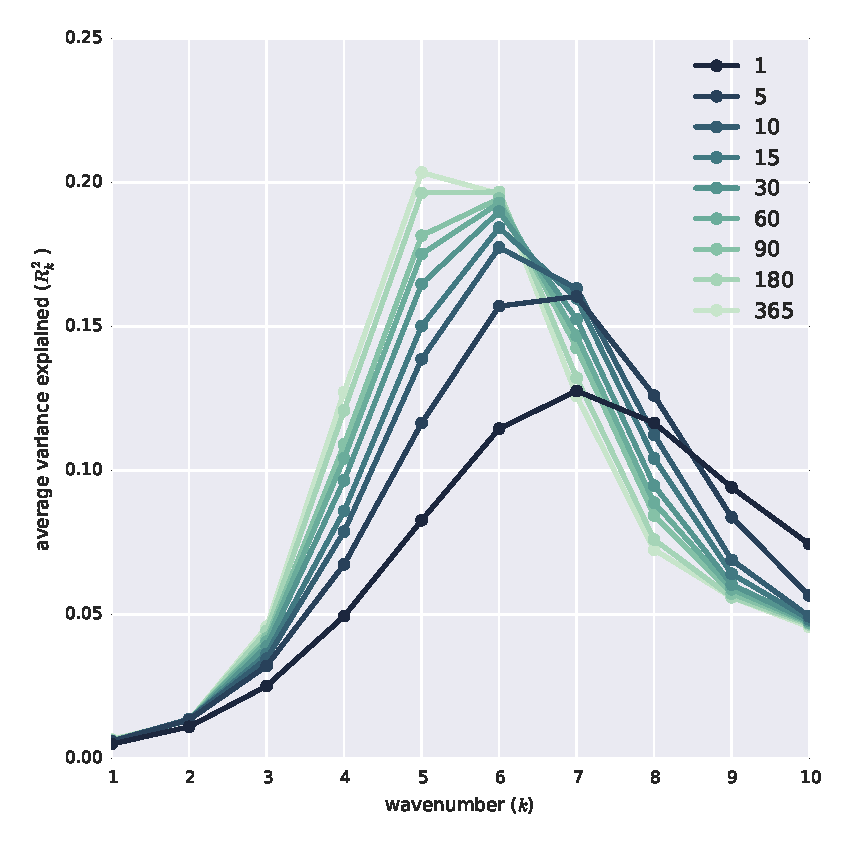
\includegraphics[width=0.7\columnwidth]{figures/psa/Figure4-3.eps}
\caption[Temporal average (1979--2014) periodograms for the meridional average (10$^{\circ}$S to 10$^{\circ}$N) 500 hPa rotated meridional wind anomaly]{\label{fig:periodogram}
Temporal average (1979--2014) periodograms for the meridional average (10$^{\circ}$S to 10$^{\circ}$N) 500 hPa rotated meridional wind anomaly (wind values outside of 115$^{\circ}$E to 235$^{\circ}$E were set to zero). Each curve represents a different running mean window that was applied to the daily timescale data prior to the analysis. The vertical axis units correspond to Equation \ref{eq:variance_explained}.%
}
\end{center}
\end{figure}


%=====================

\section{Results}

\subsection{General PSA-like variability}

Before attempting to isolate the PSA pattern using the phase information obtained from the identification algorithm, it is worth considering the characteristics of all PSA-like variability. In total, 55\% (7163 of 13120) of data times were identified as displaying PSA-like variability (i.e. wavenumber five and six were among the top three ranked frequencies), which is consistent with the fact that wavenumber six dominates the Fourier spectrum at the monthly timescale (Figure \ref{fig:periodogram}). Grouping consecutive identifications into discrete events revealed a mean event duration of 19.7 data times, with a distribution depicted in Figure \ref{fig:lifecycle}a. While interpretation of these duration data is complicated by the 30 day running mean applied to the original data (e.g. an event that lasted 10 data times could be said to span anywhere between 10 and 40 days) and the occurrence of short events immediately before or after a long event (i.e. they could conceivably be considered as a single event), it appears that PSA-like variability often persists for up to a few months at a time. Building on this baseline duration data, the life cycle of events lasting longer than 10 data times was investigated in more detail. As depicted in Figure \ref{fig:lifecycle}b, the amplitude of these events tended to peak mid-event, with some longer-lasting events peaking more than once during their lifetime (perhaps suggesting that some events simply merge into the next). The mean ($\pm$ standard deviation) linear phase trend across all events lasting longer than 10 data times was $0.12 \pm 0.38^{\circ}$E per data time, which indicates that while there was a tendency for events to propagate to the east, a substantial proportion moved very little or even towards the west during their lifetime. 

Important insights were also obtained by considering the phase distribution across all individual PSA-like data times (Figure \ref{fig:phase_distribution}). On an annual basis the distribution is clearly bimodal, with the two maxima of the kernel density estimate located at 12.75$^{\circ}$E and 45.0$^{\circ}$E. Since the phase was defined as the location of the first local maxima of the wavenumber six component of the Fourier transform, this approximate 30$^{\circ}$ phase separation indicates a pair of spatial patterns that are exactly out of phase (Figure \ref{fig:sf_composites}). Taken together these patterns clearly represent the single most dominant mode of variability in the PSA sector, and also closely resemble the PSA-1 mode identified by previous authors. On the basis of this finding, it appears that filtering the PSA-like data times according to the location of the two local maxima represents a simple and valid technique for isolating the PSA pattern from the larger population of PSA-like variability. 

The spatial patterns corresponding to the local minima of the phase distribution are also shown in Figure \ref{fig:sf_composites}, as a way to summarize the characteristics of the remaining PSA-like variability. The three anomaly centers associated with these composite mean circulation patterns have different amplitudes (the middle anomaly has a larger amplitude than the others), which indicates that it was often not a coordinated wave pattern that the identification algorithm was picking up (i.e. not the coordinated PSA-2 waveform discussed by previous authors, despite the similarity in wave phase). Looking at the individual data times corresponding to those minima (not shown), they appear to be a mixture of the hemispheric zonal wave three pattern \citep{Raphael2004,IrvingSimmonds2015}, a more meridionally oriented wave train extending from the tropical Pacific to the Amundsen Sea \citep[e.g.][]{Clem2015,Clem2015a} and isolated Amundsen Sea Low variability.


\begin{figure}
\begin{center}
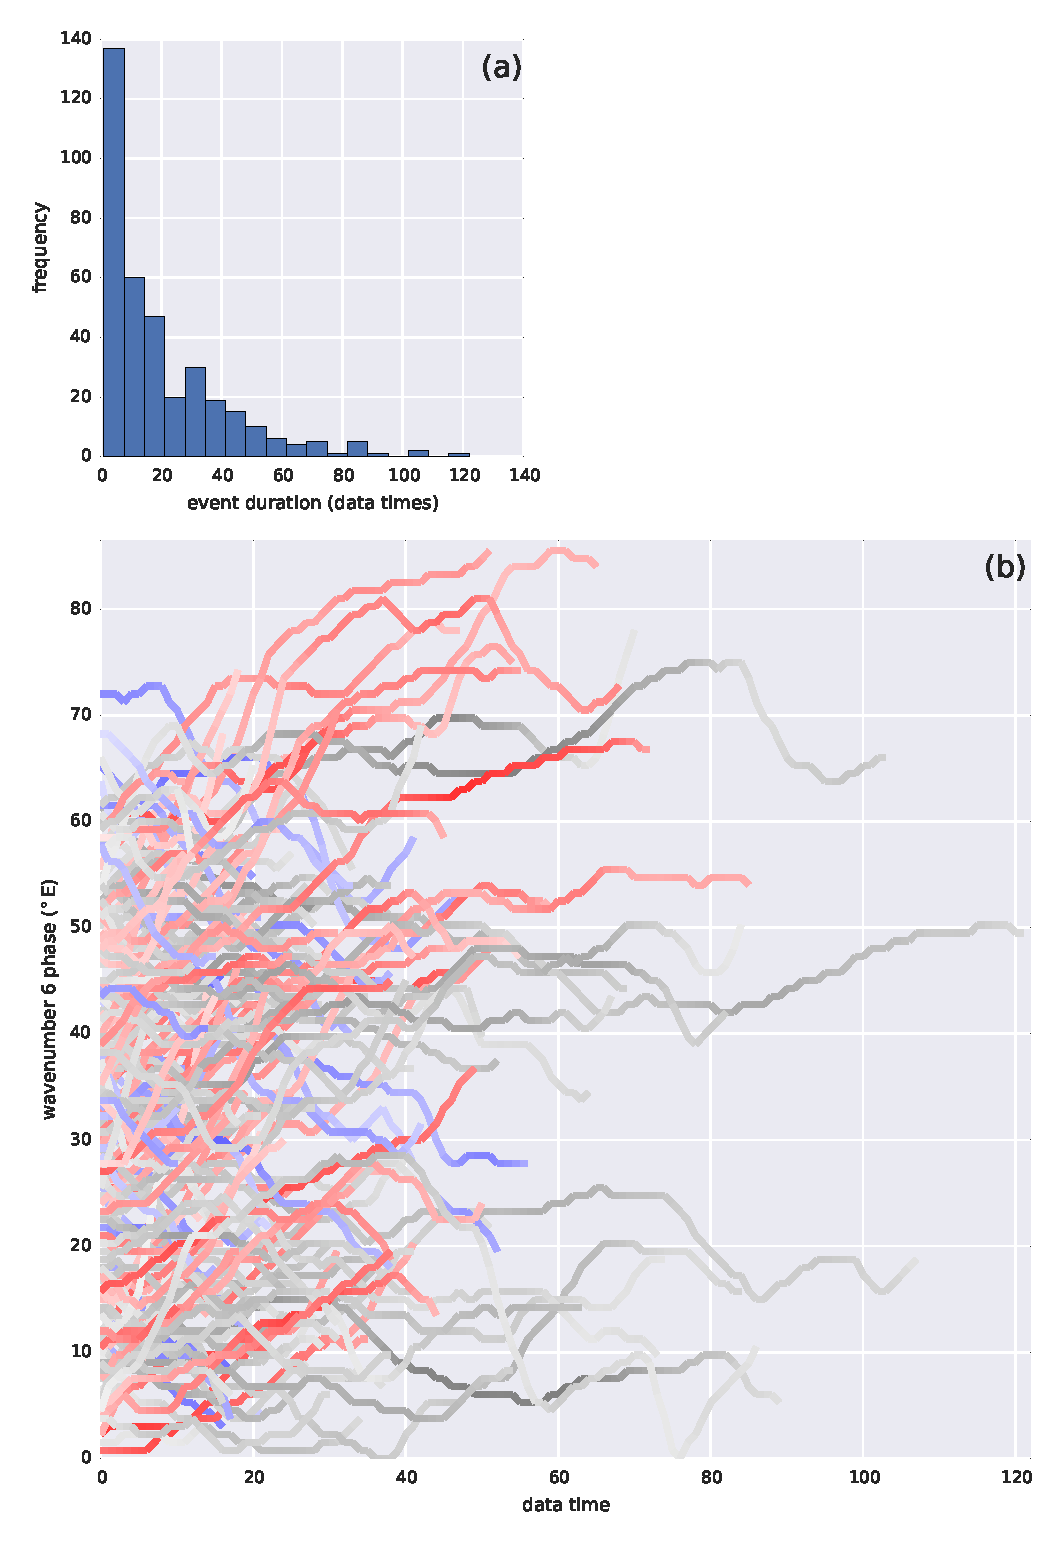
\includegraphics[width=0.8\columnwidth]{figures/psa/Figure4-4.eps}
\caption[Life cycle characteristics of PSA-like variability]{\label{fig:lifecycle}
Life cycle characteristics of PSA-like variability. The duration of all events is shown in panel (a), while the phase of events lasting more than 10 data times is shown in panel (b). Events that showed substantial eastward (defined as a linear phase gradient of greater than $0.25^{\circ}$E per data time) or westward (less than $-0.25^{\circ}$E per data time) propagation are coloured red and blue respectively, otherwise grey shading is used. The intensity of the shading represents the amplitude of the PSA-like variability. The maximum possible phase is $60^{\circ}$E, however for events that cross the cyclic 0/$60^{\circ}$E point the phase has been adjusted to ensure that a continuous line is maintained (e.g. a phase of $4^{\circ}$E would be converted to $64^{\circ}$E). %
}
\end{center}
\end{figure}

\begin{figure}
\begin{center}
\includegraphics[width=0.98\columnwidth]{figures/psa/Figure4-5.eps}
\caption[Phase distribution for all data times displaying PSA-like variability]{\label{fig:phase_distribution}
Phase distribution for all data times displaying PSA-like variability. The bars show the total count for each 0.75$^{\circ}$E interval over the period 1979--2014, while the lines represent kernel density estimates for a series of different time periods. Grey shading indicates the phase groupings taken to represent the positive (4.5 to 19.5$^{\circ}$E) and negative (37.5 to 52.5$^{\circ}$E) phase of the PSA pattern.%
}
\end{center}
\end{figure}

\begin{figure}
\begin{center}
\includegraphics[width=1\columnwidth]{figures/psa/Figure4-6.eps}
\caption[Composite mean 500 hPa streamfunction anomaly for various phase groupings]{\label{fig:sf_composites}
Composite mean 500 hPa streamfunction anomaly for four different phase groupings: positive PSA pattern (4.5 to 19.5$^{\circ}$E), minima 1 (22.5 to 37.5$^{\circ}$E), negative PSA pattern (37.5 to 52.5$^{\circ}$E) and minima 2 (50.25 to 6.0$^{\circ}$E). Dashed contours indicate negative values and the contour interval is $1.5 \times 10^6 \: m^2 s^{-1}$.%
}
\end{center}
\end{figure}


\subsection{The PSA pattern}\label{s:psa_results}

In defining the PSA pattern according to the peaks of the PSA-like phase distribution, it was necessary to account for seasonal variations in the location of those peaks (Figure \ref{fig:phase_distribution}). A spread of 15$^{\circ}$ was considered sufficient to capture these variations, and hence the 15$^{\circ}$ interval about each local maxima containing the highest mean values (taken from the annual kernel density estimate) was determined. This approach was used to account of the fact that the phase histograms were not symmetrical about the local maxima and it yielded two intervals corresponding to the positive (4.5 to 19.5$^{\circ}$E) and negative (37.5 to 52.5$^{\circ}$E) phase of the PSA pattern. Both intervals represented approximately 15\% of all data times (14.8\% for the positive phase versus 15.8\% for the negative), which suggests that the two phases have a similar frequency of occurrence. With this definition in place, it was possible to investigate variability and trends in the PSA pattern as well as its influence on surface temperature, precipitation and sea ice. 

\subsubsection{Trends and variability}

During autumn and winter in particular, the middle years of the study period (1991--2002) were characterised by a predominance of positive PSA pattern activity, while negative phase activity was more common in recent years (Figure \ref{fig:phase_distribution}). This variability is reflected in the linear trends observed over 1979--2014, with negative phase activity showing a statistically significant increasing trend (at the $p < 0.05$ level) on an annual basis and smaller non-significant increasing trends for summer, autumn and winter (Figure \ref{fig:psa-neg_seasonality}). Positive phase activity showed a non-significant decreasing trend on an annual basis and also during autumn and winter, with an increasing trend observed for summer (Figure \ref{fig:psa-pos_seasonality}). Both phases of the PSA pattern were most active during winter and spring (Figure \ref{fig:psa-neg_seasonality} and \ref{fig:psa-pos_seasonality}). 

\begin{figure}
\begin{center}
\includegraphics[width=0.9\columnwidth]{figures/psa/Figure4-7.eps}
\caption[Variability and trends in the negative phase of the PSA pattern]{\label{fig:psa-neg_seasonality}
Variability and trends in the negative phase of the PSA pattern. The total PSA-negative data times for each individual season are shown in panel (a), corresponding seasonal linear trends in panel (c) (black represents the annual trend) and monthly totals for the entire study period (1979--2014) in panel (b). To account for the fact that not all months have an equal number of days, the counts for each month in panel (b) are presented as a percentage of the total number of days for that month. Years in panel (a) are defined from December to November (e.g. the `year' 1980 spans December 1979 to November 1980) and trends that are statistically significant at the $p < 0.10$ and $p < 0.05$ level are indicated with a circle and star respectively.%
}
\end{center}
\end{figure}

\begin{figure}
\begin{center}
\includegraphics[width=0.9\columnwidth]{figures/psa/Figure4-8.eps}
\caption[Variability and trends in the positive phase of the PSA pattern]{\label{fig:psa-pos_seasonality}
As per Figure \ref{fig:psa-neg_seasonality} but for the positive phase of the PSA pattern.%
}
\end{center}
\end{figure}


In attempting to explain annual and decadal variability in the PSA pattern, previous authors have suggested that coupling between the SAM and ENSO is important \citep[e.g.][]{Fogt2006}. While some degree of coupling is evident in Figure \ref{fig:sam_v_enso} (i.e. the positive phase of the PSA pattern was most common when positive ENSO events and negative SAM events coincided), it is clear that the SAM has a much stronger association with PSA pattern activity than ENSO. Recent positive trends in the SAM during summer, autumn and to a lesser extent winter \citep[the latter being smaller and not statistically significant; e.g.][]{Simmonds2015} are also broadly consistent with the negative trends observed in the PSA pattern during those seasons.  

\begin{figure}
\begin{center}
\includegraphics[width=0.8\columnwidth]{figures/psa/Figure4-9.eps}
\caption[SAM versus Ni\~{n}o 3.4 for various temporal subsets]{\label{fig:sam_v_enso}
SAM versus Ni\~{n}o 3.4 for all data times (shown in black) over the period 1979--2014. Dots corresponding to PSA-positive and PSA-negative data times were re-coloured red and blue respectively and were arranged in the following order from front to back: blue, red, black (i.e. a blue dot might have red and/or black dots hidden underneath). For clarity, only every seventh data time was plotted. Corresponding histograms and kernel density estimates for the SAM (top panel) and Ni\~{n}o 3.4 (right panel) are shown and have been scaled according to density as opposed to frequency (hence the amplitudes are comparable).%
}
\end{center}
\end{figure}

\subsubsection{Influence on surface variables} 

In order to assess the influence of the PSA pattern on regional climate variability, the composite mean surface air temperature anomaly, precipitation anomaly and sea ice concentration anomaly was calculated for both the positive and negative phase (Figure \ref{fig:surface_composites}). On the western flank of the central composite mean streamfunction anomaly associated with positive phase activity, anomalously warm conditions were evident over the Ross Sea, Amundsen Sea and interior of West Antarctica, particularly during autumn and winter. The northerly flow responsible for these warm conditions also induced large precipitation increases along the West Antarctic coastline and reduced sea ice in the Amundsen Sea. On the eastern flank, anomalously cool conditions were evident over the Antarctic Peninsula, Patagonia and the Weddell Sea during all seasons (winter and spring especially), with the latter also experiencing large increases in sea ice. Anomalously dry conditions were also seen over the Antarctic Peninsula in association with the weaker westerly flow. 

The anomalies associated with the negative phase of the PSA pattern were essentially the reverse of the positive phase (Figure \ref{fig:surface_composites}). It is also noteworthy that while the hemispheric composite mean streamfunction anomaly associated with the PSA pattern gives the impression of a hemispheric ZW3 pattern, the phase of that pattern and the unremarkable anomalies either side of the Indian Ocean anomaly are inconsistent with the characteristics of the dominant ZW3 mode (Chapter \ref{c:zw_climatology}).

\begin{figure}
\begin{center}
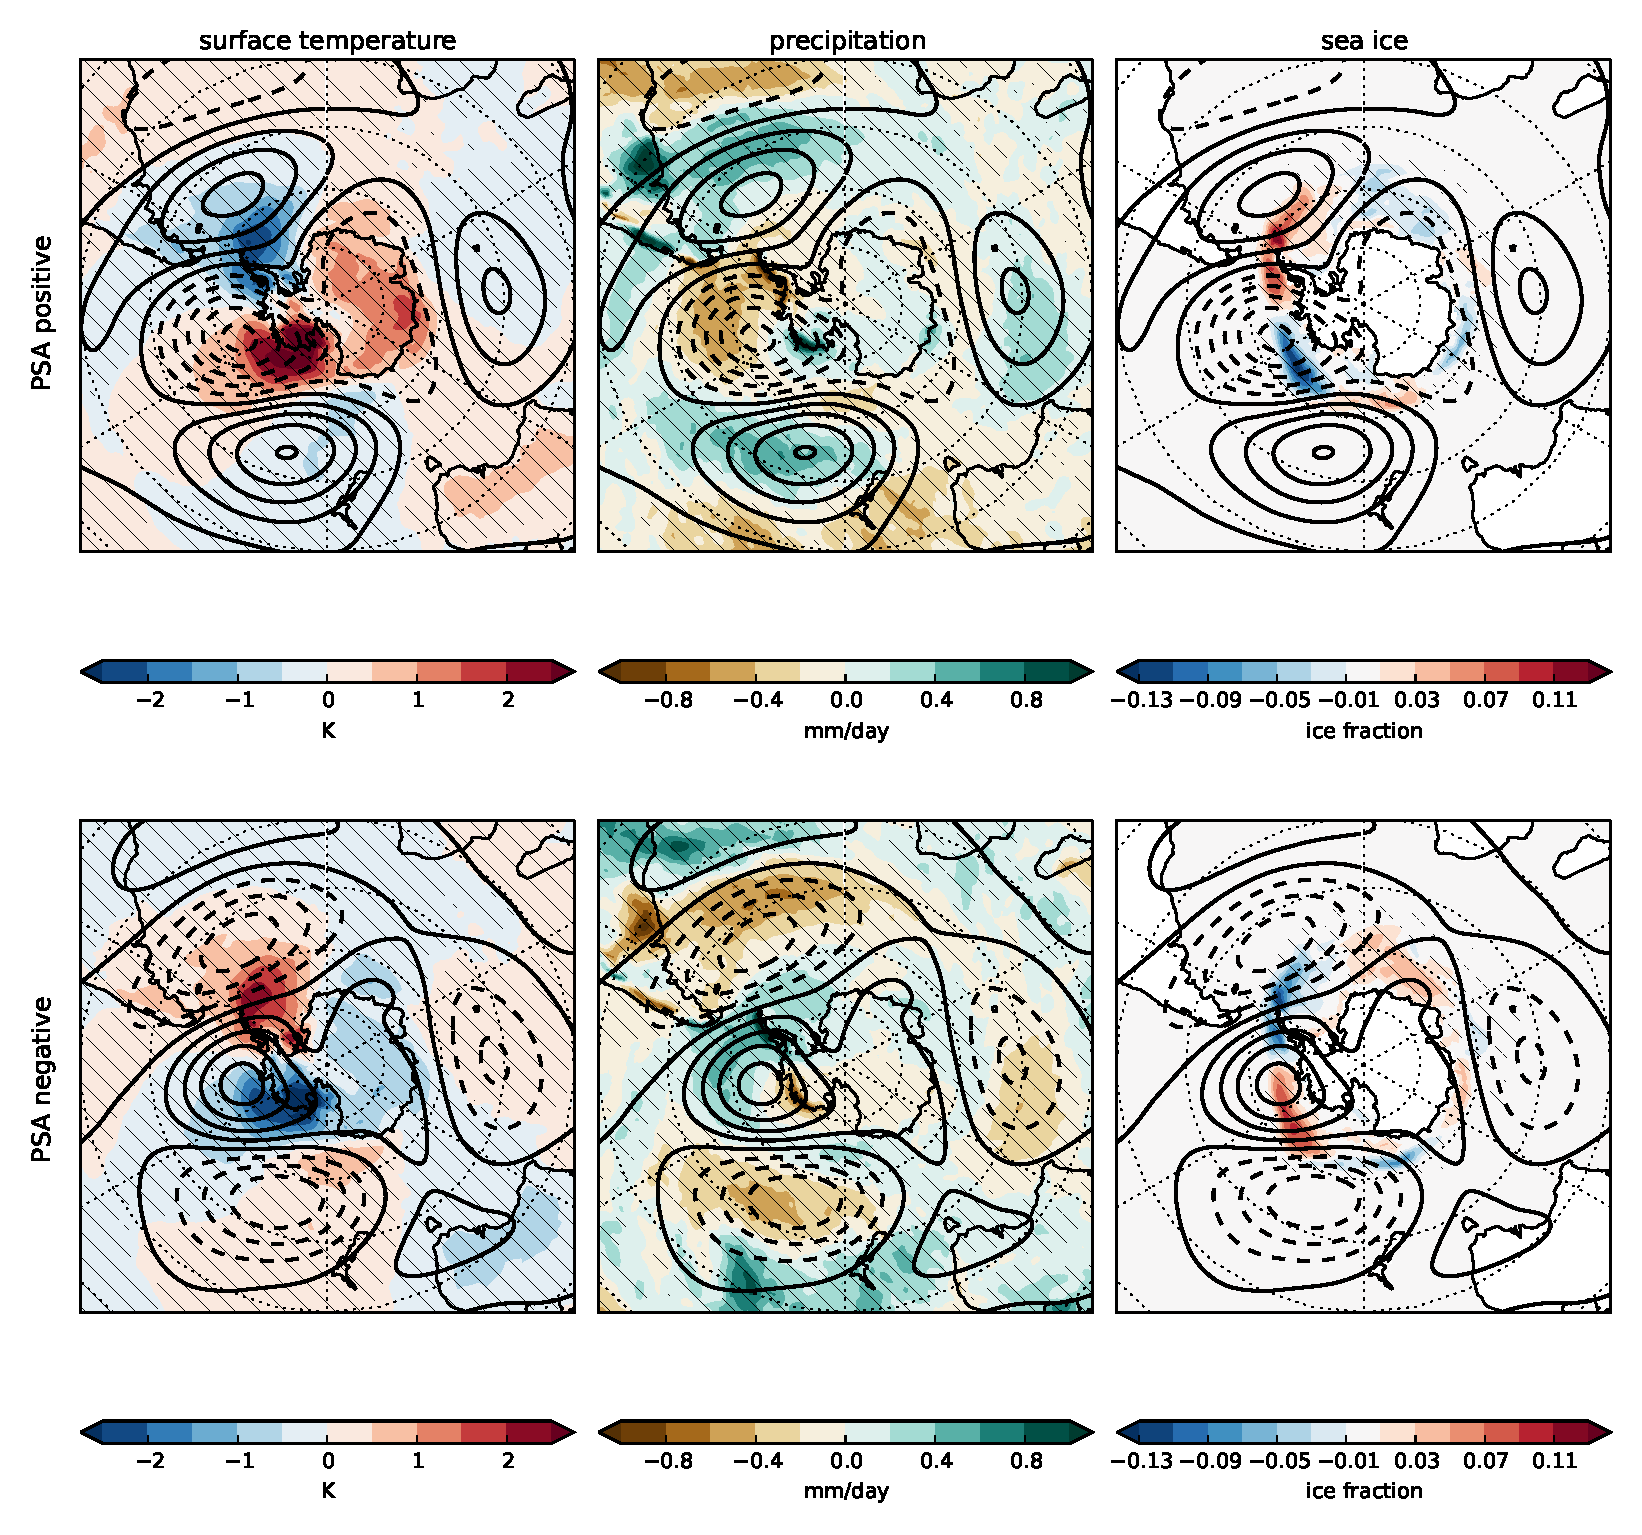
\includegraphics[width=1\columnwidth]{figures/psa/Figure4-10.eps}
\caption[Composite mean surface air temperature anomaly, precipitation anomaly and sea ice fraction anomaly for all data times corresponding to the positive or negative phase of the PSA pattern]{\label{fig:surface_composites}
Composite mean surface air temperature anomaly, precipitation anomaly and sea ice fraction anomaly for all data times corresponding to the positive (phase grouping 4.5 to 19.5$^{\circ}$E; top row) or negative (37.5 to 52.5$^{\circ}$E; bottom row) phase of the PSA pattern. Black contours show the composite mean 500 hPa streamfunction anomaly (dashed contours indicate negative values and the contour interval is $1.5 \times 10^6 \: m^2 s^{-1}$), while the hatching shows regions where the difference between the composite mean and climatological mean is significant at the $p < 0.01$ level.%
}
\end{center}
\end{figure}


%=====================

\section{Discussion}

A novel methodology has been presented for objectively identifying the PSA pattern. By rotating the global coordinate system such that the equator (a great circle path) traces the approximate path of the PSA pattern, the method was able to utilise Fourier analysis to quantify the phase and amplitude of wave-like variability in the PSA sector. In reconciling the results of this Fourier analysis with existing EOF-based definitions of the PSA pattern, a strong resemblance was found between the existing PSA-1 mode and the spatial pattern corresponding to the bimodal phase peaks of wavenumber 5--6 dominant variability in the PSA sector. The lack of a higher-order, multi-modal phase distribution questions the physical reality of the existing PSA-2 mode, and may explain the difficulty that researchers have had in identifying a tropical driver for that mode.     

These bimodal phase peaks were used as a means to define the positive and negative phase of the PSA pattern. The climatology arising from this definition revealed that the PSA pattern is most active during winter and spring, often persisting for months at a time. It propagates to the east on average, but a substantial number of events remain relatively stationary or even propagate to the west. The pattern was also shown to have a strong influence on regional temperature, precipitation and sea ice variability. With respect to the former, the results confirm existing relationships established between pattern and station temperatures over the Antarctic Peninsula \citep[e.g.][]{Schneider2012,Yu2012}, extending the regional picture to highlight equally strong temperature anomalies (of opposite sign) over West Antarctica. Large precipitation anomalies were also identified along the coast of West Antarctica and the Antarctic Peninsula, as well as over South America. These South American anomalies show a more complex spatial pattern than previous analyses (perhaps due to the higher resolution data), but are otherwise broadly consistent with the results of \citet{Mo2001}, who found the positive phase of the PSA pattern to be associated with anomalously wet conditions over southern South America and anomalously dry conditions further north. Previous studies also indicate that the PSA pattern plays an important role in sea ice variability in the Amundsen and Bellingshausen Seas \citep{Raphael2014}. The results presented here suggest that this role is not uniform across that region, with composites of the positive phase of the PSA pattern simultaneously displaying positive sea ice anomalies in the Bellingshausen Sea and negative in the Amundsen Sea.  

With respect to trends in the PSA pattern over the period 1979--2014, a trend towards the negative phase was identified on an annual basis and also during summer, autumn and winter. This autumn trend (and the high latitude temperature and sea ice anomalies associated with the negative phase of the PSA pattern) is consistent with the work of \citet{Ding2013}, who found that autumn warming over the Antarctic Peninsula and associated sea ice declines over the Bellingshausen Sea are associated with an atmospheric circulation resembling the negative phase of the PSA pattern. While this explanation makes sense on the eastern flank of the central circulation anomaly associated with that pattern, the negative phase of the PSA pattern is also associated with strong cooling over West Antarctica. Autumn temperature declines have not been observed in that region, and thus results presented here suggest that the PSA-related cooling must have been offset by other factors. 

In contrast to the autumn warming over the Antarctic Peninsula, winter warming over West Antarctica has been associated with an atmospheric circulation resembling the positive phase of the PSA pattern \citep{Ding2011}. The climatology presented here revealed a (albeit non-significant) trend towards the negative phase of the PSA pattern during winter, which raises the question: how is it that winter temperature trends over West Antarctica are associated with an atmospheric circulation resembling the positive phase of the PSA pattern, but a climatology of PSA pattern activity reveals a trend that directly opposes that finding? One possible answer to this question comes from \citet{Li2015a}. They analysed Rossby wave trains associated with observed SST trends in the tropical Atlantic, tropical Indian, west Pacific and east Pacific regions and found that all four have a center of action over the Amundsen Sea. While none of these individual wave trains resembled the PSA pattern, a linear combination of the four of them did (with the tropical Atlantic and west Pacific identified as most influential). In other words, the integrated influence of tropical SST trends on the atmospheric circulation resembles the positive phase of the PSA pattern, but the waves underpinning that teleconnection do not. This result is consistent with an earlier study that identified the tropical Atlantic as a driver of recent winter trends in West Antarctica \citep{Li2014}. Another possible answer comes from \citet{Fogt2015}, who suggest that radiative forcing has played a role in Amundsen Sea Low trends that are consistent with winter warming in West Antarctica. The absence of any springtime trend in the PSA pattern suggests that it has also not played a role in high latitude warming during that season. Similar to winter, the Atlantic has been linked to warming in West Antarctica during spring \citep{Simpkins2014}, while others point to a more meridionally oriented wave train associated with the Pacific Decadal Oscillation \citep[PDO;][]{Clem2015,Clem2015a}. 

This idea that radiatively forced Amundsen Sea Low variability and/or wave trains associated with the Atlantic or PDO might be responsible for a teleconnection resembling the PSA pattern (i.e. as opposed to changes in actual PSA pattern activity) goes to the heart of the reversibility argument made in Section \ref{s:psa_overview}. For a proposed teleconnection to be robust, it must be evident when looking through the lens of both the variable and mechanism of interest. However, even if these alternative explanations do reconcile the discrepancy between the climatology presented here and winter warming over West Antarctica, the associated circulation anomaly would bring cooler conditions and wind-driven increases in sea ice along the western Antarctic Peninsula, contrary to the observed warming and sea ice declines \citep{Clem2015}. One possible explanation is that the negative autumn sea ice anomalies persist into winter \citep{Ding2013}, however it is clear that there is still work to be done to fully understand recent winter temperature and sea ice changes in the region.

One topic not addressed here is variability in the east/west location of the PSA pattern. In response to the emergence of central Pacific ENSO events in recent years \citep[e.g.][]{Ashok2007}, some authors have suggested that the PSA pattern moves east/west depending on the precise location of the associated tropical SST anomalies \citep[e.g.][]{Sun2013,Wilson2014,Ciasto2015}. Others suggest that the pattern is relatively stationary \citep[e.g.][]{Liu2007,Ding2012}, however either way the broad region (10$^{\circ}$N to 10$^{\circ}$S in the rotated coordinate system) used by the identification algorithm developed here renders it insensitive to subtle east/west movements. Given that the PSA pattern did not show a strong association with the Ni\~{n}o 3.4 index (an index that is sensitive to both central and eastern Pacific ENSO events), it would be fair to say that even if the location of tropical SSTs does cause the pattern to move slightly, this would represent only a small fraction of all PSA pattern activity. 

This weak association with ENSO challenges our fundamental understanding of the PSA pattern. The most commonly held view to date is that the pattern is primarily a response to ENSO forcing \citep[e.g.][]{Mo2001}, whereby anomalous ENSO-related SST anomalies modify tropical convection, leading to atmospheric vorticity gradients conducive to Rossby wave generation \citep{Sardeshmukh1988}. A more comprehensive analysis of the relationship between the pattern and tropical convection would be required to confirm this (e.g. lagged correlations with SSTs and other indicators of tropical convection like the outgoing longwave radiation), but the result presented here suggest that the PSA pattern might actually be better conceptualised as a preferred regional atmospheric response to various internal and external forcings (i.e. with ENSO being just one of many players). Tropical convection is almost certainly an important factor, but its role is likely more complicated than can be captured by a broad-scale ENSO index like the Ni\~{n}o 3.4. This complex relationship between tropical SSTs, convection and the PSA pattern has been the focus of a small number of studies \citep[e.g.][]{Harangozo2004,LachlanCope2006} and is a topic that warrants much more attention. The relationship between the PSA pattern and ENSO has also traditionally been thought to be moderated by the state of the `atmospheric bridge' \citep{Liu2007}. In particular, the pattern is thought to be most active when ENSO and the SAM are in phase \citep{Fogt2006}. Rather than casting the SAM in a facilitating/bridging role, the strong association identified here is more consistent with the idea that the PSA pattern is an integral part of the zonally asymmetric structure of the SAM \citep[e.g.][]{Ding2012,Fogt2012}. 

		
\chapter{A minimum standard for publishing computational results}\label{c:reproducibility}

%=========================================================================

\begin{synopsis}
This chapter explains the rationale behind the approach taken in documenting the computational aspects of the research and considers how it might be adopted as a minimum communication standard by relevant academic journals.
\vspace{1cm}
\end{synopsis}


%===========================

The analysis of ERA-Interim data presented in the preceding chapters required the use of numerous software packages. Most of these contain many more sub-packages / libraries, which together perform a specific task such as data visualisation, EOF analysis, spherical grid rotation or manipulation of netCDF file attributes. A major component of the research therefore involved writing (many thousands of lines of) code to link these packages and sub-packages into a coherent data analysis workflow. For parts of the workflow where no ready-made software package existed, it was also necessary to write a new package / function for that task (e.g. a new Hilbert transform function was written by combining pre-existing Fourier analysis routines from the SciPy library).

Given the computationally intensive nature of this data analysis, it would be impossible for another researcher to reproduce the results without details of the software and code. This is true of essentially all contemporary weather and climate science, and yet traditional academic publishing formats and conventions do not allow for the documentation of these aspects of the research methodology. As discussed in Section \ref{s:reproducibility_overview}, the absence of adequate software and code documentation, along with other issues such as access to research data, has led to something of a reproducibility crisis in modern computational research \citep[e.g.][]{Peng2011}. 

In order to ensure the reproducibility of the zonal wave and PSA pattern analyses presented in this thesis, a comprehensive procedure was devised for documenting the computational aspects of a research project. In the first instance, this involved a broad consultation of the literature to find out (a) why researchers do not currently publish their code, and (b) what computational best practices they should follow when they do. An approach was then designed (and implemented in Section \ref{s:computation} and the journal publications arising from the thesis) that sought to reduce the barriers for researchers, while at the same time promoting established best practices in scientific computing. In order to stimulate further discussion and progress in the area of reproducibility, this approach was then used as a starting point for defining a minimum communication standard that could be adopted by journals in the weather and climate sciences, as well as a set of lesson materials aimed at researchers wanting to learn the skills required to adhere to those standards. 

The details of the literature review (Section \ref{s:reproducibility_review}), rationale behind the procedure for documenting the computational aspects of a research project (Section \ref{s:reproducibility_approach}), proposed minimum communication standard (Section \ref{s:reproducibility_standards}) and lesson materials (Section \ref{s:reproducibility_lessons}) are documented in this chapter.


%===========================

\section{Literature review}\label{s:reproducibility_review}

The literature on the topic of barriers to publishing code is relatively sparse, however a recent survey of the machine learning community found that the top reason for not sharing code was the perceived time required to prepare it for publication, followed by the prospect of dealing with questions from users \citep{Stodden2010}. While many researchers are sympathetic to the ideals of open science and reproducible research, it appears that the practicalities seem too difficult and time consuming, particularly when the pressure to publish is so strong and unrelenting. The vast majority of survey respondents also identified as self-taught programmers, which suggests that the computational competency of the community is relatively low. 

While there are numerous scientific best practices documented in the literature \citep[e.g.][]{Wilson2014a}, only a few are directly relevant to the documentation of reproducible research. The first is that researchers should be saving the commands used to produce a particular result in a file (called a script), so that the sequence of commands can be repeated at a later time. While this best practice is something that most weather and climate scientists are comfortable with, it is important to note that authors should not aim to produce a single script for each key result. This is because a second relevant best practice is that of modularising code, rather than copying and pasting. Since duplication of any segment of code is error prone (because updates would need to be applied multiple times), researchers should instead aim to develop a whole library/repository of code containing many interconnected scripts (i.e. that each import key code segments from elsewhere). The revision history of that repository can then be tracked using a version control system like Git, Subversion or Mercurial, so that previous versions can be easily retrieved (e.g. to find out exactly what commands were used to produce a particular figure that was generated six months ago). These version control systems are easily linked to an online hosting service such as GitHub or Bitbucket, which is the means by which a code repository can be made publicly available.

Besides these core best practices, the literature points to a wide range of tools for assisting with reproducibility. While these tools are no doubt proposed with good intentions, the bewildering array of options is one reason why an individual working in the weather and climate sciences might place reproducibility in the `too hard' basket. An appropriate solution for any given scientist no doubt exists within that collection of tools, but it is heavily obscured. Consider the `regular' scientist described in Box \ref{box:regular_scientist}. In consulting the literature on reproducible computational research, they would be confronted with options including data provenance tracking systems like VisTrails \citep{Freire2012} and PyRDM \citep{Jacobs2014}, software environment managers like Docker and Vagrant \citep{Stodden2014}, and even online services like RunMyCode.org where your code and data can be run by others \citep{Stodden2012}. These might be good options for small teams of software engineers or experienced scientific programmers dealing with very large workflows (e.g. the post-processing of thousands of model runs), complex model simulations and/or production style code (e.g. they might be developing a satellite retrieval algorithm that has high re-use potential in the wider community), but a regular scientist has neither the requisite computational experience or a research problem of sufficient scale and complexity to necessarily require and/or make use of such tools. The procedure outlined below was designed with this regular scientist in mind. It looked to minimise both the time involved and the complexity of the associated tools, while at the same time remaining faithful to established best practices in scientific computing.


\begin{featurebox}

\begin{tcolorbox}[width=\textwidth]

The procedure for documenting computational results outlined in this chapter was developed with a `regular' weather/climate scientist in mind. A characterisation of this scientist is given below and is based on the few documented surveys of how computational scientists do their work \citep{Hannay2009,Stodden2010,Momcheva2015}, editorials describing current computational practices \citep[e.g.][]{Easterbrook2014} and the author's personal experience teaching at numerous Software Carpentry workshops over the past few years (Section \ref{s:reproducibility_lessons}). This regular scientist:
\begin{itemize}
\item Works with publicly available data (e.g. reanalysis data) that is often large in size (e.g. it might be tens or hundreds of gigabytes), but is not so large as to be considered `big data.' 
\item Acquired the knowledge to develop and use scientific software from peers and through self-study, as opposed to formal education and training.
\item Primarily relies on software like Python, MATLAB, IDL, NCL or R, which has a large user/support base and is relatively simple to install on a Windows, Mac or Linux computer.
\item Does most of their work on a desktop or intermediate computer (as opposed to a supercomputer).
\item Is only writing code for a specific task/paper and is not looking for community uptake.  
\item Works on their own or in a very small team (e.g. 2--3 other scientists) and does not have access to professional software developers for support.
\end{itemize}

Some scientists might be regular in most but not all aspects of their work (e.g. all the points above might apply except they occasionally use a highly specialised software package that does not have a large support base) so this characterisation can be thought of as a baseline or minimum level of computation that essentially all weather and climate scientists are engaged in.  

\end{tcolorbox}

\caption{\label{box:regular_scientist}
Description of a regular scientist.}
\end{featurebox}


%===========================  
  
\section{Documenting the computational aspects of a research project}\label{s:reproducibility_approach}

At first glance, the only difference between a regular thesis or journal article and that presented here is the addition of a short computation section (e.g. Section \ref{s:computation}). That section accompanies the traditional description of data and methods and briefly cites the major software packages used in the research, before pointing the reader to three key supplementary items: (1) a more detailed description of the software used, (2) a version controlled and publicly available code repository and (3) a collection of supplementary log files that capture the data processing steps taken in producing each key result. The repository was hosted at a popular code sharing website called GitHub, while the detailed software description and log files were hosted at Figshare \citep{IrvingFigshare2016}, which is a website where researchers commonly archive the `long tail' of their research (e.g. supplementary figures, code and data). 

\subsection{Software description}

There is an important difference between citing the software that was used in a study (so that authors get appropriate academic credit) and describing it in sufficient detail so as to convey the precise version and computing environment \citep{Jackson2012}. Recognising this, the computation section should begin with a high-level description of the software used, which includes citations to any papers written about the software. Authors of scientific software are increasingly publishing with journals like the \textit{Journal of Open Research Software}, so it is important for users of that software to cite those papers within their manuscripts. This high-level description is also useful for briefly articulating what general tasks each software item was used for (e.g. plotting, data analysis, file manipulation). Such an overview does not provide sufficient detail to recreate the computing environment used in the study, so it is also necessary to provide a link to a supplementary file that documents the precise version of each software package used and the operating system upon which it was run (namely the name, version number, release date, institution and DOI or URL; Box \ref{box:software_description}). 

\begin{featurebox}

\begin{tcolorbox}[width=\textwidth]

\begin{lstlisting}[basicstyle=\footnotesize\ttfamily, breaklines=true]
Operating system: 

Ubuntu. 12.04. April 2012. Canonical Ltd.
    http://www.ubuntu.com/

Software packages:

netCDF Operators. 4.4.6. September 2014. netCDF Operators Project.
    http://sourceforge.net/projects/nco/
Climate Data Operators. 1.7.0. October 2015. Max Plank Institut fur Meteorologie. Hamburg, Germany. 
    https://code.zmaw.de/projects/cdo
Anaconda. 2.0.1. July 2014. Continuum Analytics. Austin, Texas.
    http://docs.continuum.io/anaconda/
Python. 2.7.10. May 2015. Python Software Foundation.
    https://www.python.org/
NumPy. 1.10.1. October 2015. NumPy Developers. 
    http://www.numpy.org/
SciPy. 0.16.0. July 2015. SciPy Developers.
    http://www.scipy.org/scipylib/
xray. 0.5.1. June 2015. xray Developers.
    http://xray.readthedocs.org/
windspharm. 1.3.1. June 2014. Andrew Dawson.
    http://ajdawson.github.io/windspharm/
eofs. 0.5.0. June 2014. Andrew Dawson.
    http://ajdawson.github.io/eofs/
pyqt_fit. 1.3.3. August 2014. Pierre Barbier de Reuille. 
    https://pyqt-fit.readthedocs.org/
matplotlib. 1.4.3. July 2015. Matplotlib Development Team.
    http://matplotlib.org/
seaborn. 0.6.0. June 2015. Michael Waskom.
    http://stanford.edu/~mwaskom/software/seaborn/
iris. 1.8.1. June 2015. Met Office. Exeter, England.
    http://scitools.org.uk/
cartopy. 0.13.0. June 2015. Met Office. Exeter, England.
    http://scitools.org.uk/
\end{lstlisting}

\end{tcolorbox}

\caption{\label{box:software_description}
Software environment used in producing the results presented in this thesis \citep[and documented at][]{IrvingFigshare2016}.}

\end{featurebox}  

\subsection{Code repository}

Most of the examples of reproducible research currently available in the literature produce a pristine GitHub or Bitbucket repository for their paper (i.e. one that only contains code directly relevant to that paper), however this should not be an expectation for regular scientists who are not looking for broad-scale community uptake of their code. Not only is this a time consuming practice that would likely involve a degree of cutting and pasting, it also goes against the workflow that version control promotes. By providing a link to their everyday repository instead, authors can quickly and easily signal to readers what code was used to produce the results in their paper. The authors may further develop that code in the future, so the reader then also has easy access to the latest version if they would like to use it in their own work and/or suggest improvements (referred to as a `pull request' in version control parlance). There are all sorts of extra bits and pieces of code in the everyday repository that is linked to in Section \ref{s:computation}. Readers will probably never look at that code (because it is not referred to in the associated log files), but what is the harm if they do? Students and other scientists could potentially learn from it, and in the best case scenario they would inform the author of a bug or potential improvement to the code.        

In addition to providing a link to the associated Github repository, this thesis provides \citep[on Figshare;][]{IrvingFigshare2016} a static snapshot of the repository taken at the time of publication. The motivation for doing this was to ensure that a static version of the code is available in case the associated GitHub repository is ever moved or deleted. Unlike GitHub, archiving sites such as Figshare and Zenodo issue DOIs, which function as a perpetual link to the resource and can only be obtained by agencies that commit to maintain a reliable level of preservation \citep{Potter2015}. Since this snapshot does not provide a revision history of the code, it would not have been appropriate to provide it \textit{instead} of the link to GitHub. Not all of the results presented in a research paper or thesis will necessarily have been generated with the very latest version of the code, hence the need for the revision history (and even if they were generated with the latest version, it is not possible to submit a pull request to Figshare or Zenodo). Both Figshare and Zenodo provide a simple interface for importing code directly from GitHub, so the process is very straightforward.

\subsection{Log files}\label{s:log_files}

A code repository and software description on their own are not much use to a reader; they also need to know how that code was used in generating the results presented. It turns out that in the weather and climate sciences, the answer to adequately documenting the computational steps involved in producing a given result has been staring us in the face for years. As a community we have almost universally adopted a self-describing file format (i.e. a format where metadata can be stored within the file) called network Common Data Form (netCDF), which means we have been able to develop numerous software tools for processing and manipulating data stored in that format. The most well known of these are a collection of command line tools known as the NetCDF Operators (NCO) and Climate Data Operators (CDO). Whenever an NCO or CDO command is executed, a time stamp followed by a copy of the command line entry is automatically placed into the global attributes of the output netCDF file, thus maintaining a history of the provenance of that data (see Box \ref{box:log_file} for examples of NCO and CDO entries).

What is important here is not the specific software tools or file format (there are many researchers who do not use NCO, CDO, or netCDF files) but rather the deceptively simple method for recording previous computational steps. Using any of the programming languages common to the weather and climate sciences, a user can obtain details of the associated command line entry and append such text to the global attributes of a netCDF file (or a corresponding metadata text file if dealing with file formats that are not self-describing). In fact, in all of these languages such tasks can be achieved with just a few lines of additional code. This thesis provides a log file containing a complete NCO/CDO-style history for each figure; see Box \ref{box:log_file} for details of one of those files and the associated page on Figshare \citep{IrvingFigshare2016} for the complete set.

An important feature of these log files is that they are both readable and writable by any weather and climate scientist. If advanced practitioners are tracking their computational steps with tools like VisTrails then they can certainly submit log files (or equivalent documentation) exported from those tools, but as a minimum standard it is important that elaborate tools are not a requirement. By spelling out every single computational step (i.e. from initial data download to the final plot/result), the log files also ensure that readers do not need to be familiar with build tools like Make or other workflow management tools in order to figure out which computational steps were executed and in what order. Other features of note include:
\begin{itemize}
\item Besides a slight amendment to the initial download entry of the log file shown in Box \ref{box:log_file} (the default text provided by the ERA-Interim data server was not particularly self explanatory), no manual editing of its contents was done. This means that if a reviewer asked for a slight modification to the figure, for instance, the regeneration of a new log file would be trivial. By resisting the urge to clean up the file (e.g. one might consider removing path details) it also doubles as a record that is highly useful to the author in retracing their own steps (e.g. they could use it to recall where they stored the output data on their local machine).
\item As previously mentioned, it cannot be assumed that the latest version of any code repository was used to generate all the results in a given paper. The unique version control revision number (known as a hash value) was therefore recorded in the log files, wherever a script written by the author was executed. Languages like Python, R and MATLAB are able to link with version control systems like Git, so the retrieval of the revision number can be automated.
\item When more than one input file is passed to an NCO or CDO function, the history of only one of those files is retained in the output file. On occasions where this is not appropriate (i.e. where the histories of the multiple input files are very different), it is important to ensure that the history of all input files is retained. There are a number of examples of this in the log files provided on Figshare. 
\end{itemize}
  
 
 \begin{featurebox}

\begin{tcolorbox}[width=\textwidth]

\begin{lstlisting}[basicstyle=\footnotesize\ttfamily, breaklines=true]
Mon Nov 16 09:11:28 2015: /usr/local/anaconda/bin/python /home/STUDENT/dbirving/climate-analysis/visualisation/plot_hilbert.py /mnt/meteo0/data/simmonds/dbirving/ERAInterim/data/va_ERAInterim_500hPa_030day-runmean_native.nc va /mnt/meteo0/data/simmonds/dbirving/ERAInterim/data/zw/figures/hilbert_zw_w19_va_ERAInterim_500hPa_030day-runmean_native-55S_1986-05-22_2006-07-29.eps 1 2 --latitude -55 -55 --dates 1986-05-22 2006-07-29 --wavenumbers 1 9 --figure_size 15 6 --envelope 1 9 (Git hash: a9573e4)

Tue Jun 30 07:35:49 2015: cdo runmean,30 /mnt/meteo0/data/simmonds/dbirving/ERAInterim/data/va_ERAInterim_500hPa_daily_native.nc /mnt/meteo0/data/simmonds/dbirving/ERAInterim/data/va_ERAInterim_500hPa_030day-runmean_native.nc

Wed Mar 18 17:17:14 2015: cdo mergetime va_ERAInterim_500hPa_daily-2014-06-01-to-2014-12-31_native.nc ../data/va_ERAInterim_500hPa_daily_native_orig.nc ../data/va_ERAInterim_500hPa_daily_native.nc

Mon Nov 10 17:15:49 2014: ncatted -O -a level,va,o,c,500hPa va_ERAInterim_500hPa_daily_native.nc

Mon Nov 10 16:31:05 2014: ncatted -O -a long_name,va,o,c,northward_wind va_ERAInterim_500hPa_daily_native.nc

Thu Aug 21 10:57:46 2014: ncatted -O -a axis,time,c,c,T va_ERAInterim_500hPa_daily_native.nc

Thu Aug 21 10:34:46 2014: ncrename -O -v v,va va_ERAInterim_500hPa_daily_native.nc

Thu Aug 21 10:26:49 2014: cdo invertlat -sellonlatbox,0,359.9,-90,90 -daymean va_ERAInterim_500hPa_6hourly_native.nc va_ERAInterim_500hPa_daily_native.nc

Thu Aug 21 10:14:59 2014: cdo mergetime ../download/va_ERAInterim_500hPa_6hourly-1979-1988_native_unpacked.nc ../download/va_ERAInterim_500hPa_6hourly-1989-1998_native_unpacked.nc ../download/va_ERAInterim_500hPa_6hourly-1999-2008_native_unpacked.nc ../download/va_ERAInterim_500hPa_6hourly-2009-2014_native_unpacked.nc va_ERAInterim_500hPa_6hourly_native.nc

Thu Aug 21 10:13:35 2014: ncpdq -P upk va_ERAInterim_500hPa_6hourly-2009-2014_native.nc va_ERAInterim_500hPa_6hourly-2009-2014_native_unpacked.nc

Wed Aug 20 23:16:22 2014: Initial download of 6 hourly, 500 hPa meridional wind ERA-Interim data in 5 or 10 year chunks (e.g. va_ERAInterim_500hPa_6hourly-2009-2014_native.nc) from http://apps.ecmwf.int/datasets/data/interim-full-daily/
\end{lstlisting}

\end{tcolorbox}

\caption{\label{box:log_file}
Log file corresponding to Figure \ref{fig:example_hilbert}. Details regarding the software and code referred to in the log file are provided in Section \ref{s:computation}.}

\end{featurebox}  
 
 
%===========================

\section{A formal minimum standard}\label{s:reproducibility_standards}

\subsection{Implications and practicalities}

Before formally proposing a minimum standard for the communication of computational results, it is worth considering the implications and practicalities of adopting a standard based on the approach described above. The reproducibility of published results would presumably improve, which may also lead to increased trust, interest and citations \citep{Piwowar2007}, but what else would it mean for authors and reviewers? Would there be barriers to overcome in implementing such a standard, and what could be done to make the transition easier?

\subsubsection{Authors}

As previously mentioned, \citet{Stodden2010} identified the time involved as the largest barrier to sharing code. There are numerous authors who argue that the best practices like scripting and version control save time in the long run \citep[e.g.][]{Sandve2013,Wilson2014a} and objective evidence is beginning to emerge in support of this claim \citep{Simperler2015}. This means that once researchers have learned and adopted these practices, they may actually save time. In the author's experience as a Software Carpentry instructor (Section \ref{s:reproducibility_lessons}), many weather and climate scientists are comfortable with the idea of scripting, but very few use version control. Learning these new skills is not overly time consuming (Software Carpentry teaches them in a short two-day workshop), but on a local level it requires an individual or institution to take the lead in liaising with Software Carpentry to find volunteer instructors and to coordinate other logistics. A good example is the Australian Meteorological and Oceanographic Society (AMOS), which has hosted a Software Carpentry workshop alongside its annual conference for the past three years running. Of course, it is also possible to learn these skills by following an online tutorial (e.g. all the Software Carpentry lessons are available online), but there is an added benefit to the social aspect of a workshop. It helps to reduce the embarrassment many scientists have about the quality of their code (i.e. they see that their peers are no `better' at coding than they are), which is an important part of achieving the required cultural shift towards an acceptance of code sharing \citep{Barnes2010}.

The other potentially time consuming task associated with adopting a minimum standard would be dealing with requests for assistance. One suggested solution to this problem is to make it clear that authors are not obliged to support others in repeating their computations \citep{Easterbrook2014}. This is probably the only feasible solution, but it is worth noting that even if not formally obliged, some authors may fear that refusing requests will make it look like they are uncooperative and/or have something to hide. 

Some researchers also face barriers relating to security and proprietary, particularly if they are using large code bases that have been developed for research and/or operations within government laboratories, national weather bureaus and private companies \citep{Stodden2010}. Such code bases are increasingly being made public (e.g. the Australian Bureau of Meteorology and CSIRO host the code for their Climate and Weather Science Laboratory in a public GitHub repository), but any proposed minimum standard would need to allow some flexibility for researchers who are unable to make their code public for these reasons (the code archived by MPI-M is available via request only, which might be an acceptable solution in many cases). For those concerned about getting appropriate academic credit for highly novel and original code, a separate publication (e.g. in the \textit{Journal of Open Research Software}) or software license \citep[e.g.][]{Morin2012} might also be an option.

\subsubsection{Reviewers}

In requiring authors to make their code available, it would be important to convey to reviewers that they are not expected to review the code associated with a submission; they simply have to check that it is sufficiently documented (i.e. that the code is available in an online repository and that log files have been provided for all figures and key results). Not only would it be unrealistic to have reviewers examine submitted code due to the wide variety of software tools and programming languages out there, it would also be inconsistent with the way scientific methods have always been reviewed. For instance, in the 1980s it was common for weather and climate scientists to manually identify weather systems of interest (e.g. polar lows) from satellite imagery. The reviewers of the day were not required to go through all the satellite images and check that the author had counted correctly, they simply had to check that the criteria for polar low identification was adequately documented. This is not to say that counting errors were not made on the part of authors (as with computer code today there were surely numerous errors/bugs), it was just not the job of the reviewer to find them. Author errors are revealed when other studies show conflicting results and/or when other authors try to replicate key results, which is a process that would be greatly enhanced by having a minimum standard for the communication of computational results. This idea of conceptualising the peer review of code as a post publication process is consistent with the publication system envisaged by the open evaluation movement \citep[e.g.][]{Kriegeskorte2012}. 
  
\subsection{Proposed standards}

To assist in establishing a minimum standard for the communication of computational results, it is proposed that the following text (or something in the same spirit) could be inserted into the author and reviewer guidelines of journals in the weather and climate sciences (institutions that have their own internal review process could also adopt these guidelines). In places the language borrows from the guidelines recently adopted by \textit{Nature} \citep{Nature2014}. It is anticipated that a journal would provide links to examples of well documented computational results to help both authors and reviewers in complying with these guidelines. The journal could decide to host the supplementary materials itself (i.e. the software description, log files and static snapshot code repository), or encourage the author to host these items at an external location that can guarantee persistent, long-term access (e.g. an institutionally supported site like MPI-M provides for its researchers or an online academic archive such as Figshare or Zenodo).

\subsubsection{Author guidelines}

If computer code is central to any of the paper's major conclusions, then the following is required as a minimum standard: 
\begin{enumerate}
\item A statement describing whether (and where) that code is available and setting out any restrictions on accessibility. 
\item A high-level description of the software used to execute that code (including citations for any academic papers written to describe that software).
\item A supplementary file outlining the precise version of the software packages and operating system used. This information should be presented in the following format: name, version number, release date, institution, DOI or URL.
\item A supplementary log file for each major result (including key figures) listing all computational steps taken from the initial download/attainment of the data to the final result (i.e. the log files describe how the code and software were used to produce the major results). 
\end{enumerate}

It is recommended that items 1 and 2 are included in a `Computation' (or similarly named) section within the manuscript itself. Any practical issues preventing code sharing will be evaluated by the editors, who reserve the right to decline a paper if important code is unavailable. While not a compulsory requirement, best practice for code sharing involves managing code with a version control system such as Git, Subversion or Mercurial, which is then linked to a publicly accessible online repository such as GitHub or Bitbucket. In the log files a unique revision number (or hash value) can then be quoted to indicate the precise version of the code repository that was used. Authors are not expected to produce a brand new repository to accompany their paper; an `everyday' repository which also contains code not relevant to the paper is acceptable. Authors should also note that they are not obliged to support reviewers or readers in repeating their computations.

\subsubsection{Reviewer guidelines}

The reviewer guidelines for most journals already ask if the methodology is explained in sufficient detail so that the paper's scientific conclusions could be tested by others. Such guidelines could simply be added to as follows: `If computer code is central to any of those conclusions, then reviewers should ensure that the authors are compliant with the minimum standards outlined in the author guidelines. It should be noted that reviewers are not obliged to assess or execute the code associated with a submission. They must simply check that it is adequately documented.'   


%===========================  

\section{Software Carpentry lesson materials}\label{s:reproducibility_lessons}

Software Carpentry is a volunteer organisation whose members teach basic programming skills to researchers in science, engineering and medicine \citep{Wilson2014}. Over the past few years it has run hundreds of two-day workshops at research institutions around the world and is now a global leader in computing education. One key to the success of the organisation has been the fact that most qualified Software Carpentry instructors are research scientists as opposed to professional software developers. This avoids a well-known teaching phenomenon called expert blind spot; the instructors can remember what it is like not to understand basic programming concepts and are able to write scientist-appropriate lesson materials.

As part of the 2013 AMOS conference in Melbourne, Greg Wilson (the founder of Software Carpentry) flew to Australia to run a workshop for the AMOS community. Like all Software Carpentry workshops, it delivered lessons on automating tasks using the Unix shell, structured programming in Python (including how to write programs that are executable at the command line) and version control using Git. While these are all the basic skills required to adhere to the proposed communication standards, it was felt that an additional `capstone' lesson was required to pull all those skills together into a coherent example specific to the weather and climate sciences. Over the next few months the author completed the Software Carpentry instructor training course and developed this capstone lesson \citep{IrvingSWC2015}, before delivering it and the rest of the core Software Carpentry materials at a workshop alongside the 2014 AMOS conference in Hobart (and again at the 2015 conference in Brisbane). Importantly, that lesson describes how to create the log files discussed in Section \ref{s:log_files}. 


%===========================

\section{Discussion}

In order to combat the reproducibility crisis in published computational research, a simple procedure for communicating computational results has been demonstrated and its rationale discussed. The procedure involves authors providing three key supplementary items: (1) a description of the software packages and operating system used, (2) a (preferably version controlled and publicly accessible) code repository, and (3) a collection of supplementary log files that capture the data processing steps taken in producing each key result. It should provide a starting point for weather and climate scientists (and perhaps computational scientists more generally) looking to publish reproducible research, and could be adopted as a minimum standard by relevant academic journals.

The procedure/standard was developed to be consistent with recommended computational best practices and seeks to minimise the time burden on authors, which has been identified as the most important barrier to publishing code. In particular, best practice dictates that at a minimum weather and climate scientists should be (a) writing data analysis scripts so they can re-run their analyses, (b) using version control to manage those scripts for backup and ease of sharing/collaboration and (c) storing the details of their analysis steps in the global history attribute of their netCDF data files (or following an equivalent process for other file formats) to ensure the complete provenance of their data. In order to make their published results reproducible, it follows that the minimum an author would need to do is simply make those history attributes available (via log files) along with the associated code repository and a description of the software used to execute that code. The attainment of this minimum standard would involve a slight change to the workflow of many regular weather and climate scientists (e.g. most do not use version control), however the standard has been designed to only require skills that can be learned very quickly (e.g. at a two-day Software Carpentry workshop).  

While widespread adoption of this minimum standard would be a great starting point for reproducible research, it is worth noting that as a community we should ultimately aim much higher. By way of analogy, minimum standards in the construction industry ensure that buildings will not fall over or otherwise kill their inhabitants, but if everyone only built to those minimum standards our cities would be hugely energy inefficient. The proposed minimum standard for computational research ensures that published results are reproducible (which is a big improvement on the current state of affairs), but recreating workflows from the log files, daily code repositories and software descriptions of even just moderately complex analyses would be a tedious and time consuming process. Once comfortable with the skills and processes required to meet the minimum standard, authors should seek to go beyond them to improve the comprehensibility of their published computational results, in the same way that builders should strive for a five-star energy rating. The precise tools and methods used in this endeavour will vary from author to author; basic analyses might only require the inclusion of informative REAMDE files that explain in plain language how to execute the code, while others might choose to provide informative flow diagrams exported from provenance tracking systems like VisTrails, pre-package their code/software for ease of installation (e.g. for inclusion in the Python Package Index) and/or make their software environment available via Docker. As previously mentioned, it would not be appropriate to include these many varied (and often complex) options in any minimum standards, but they represent an excellent next-step for scientists who have mastered the basics and will hopefully see more uptake as the computational competency of the community improves over time.

  








		
\chapter{Conclusions}

%=========================================================================

\begin{synopsis}

The chapter summarises the major contributions of the thesis, including a discussion of the associated limitations and directions for further research.

\end{synopsis}

%=======================

\section{New approaches to wave identification}

The first major contribution of the thesis is the new approaches it presents for the identification and characterisation of long-lived, quasi-stationary waveforms. By adapting data analysis techniques from related fields of research (i.e. the wave envelope construct used in identifying synoptic-scale Rossby wave packets and a grid rotation method commonly used in ocean modelling) these approaches fully exploit the capabilities of Fourier analysis, thus allowing a more complete description of the waveform characteristics (e.g. wave phase and amplitude). A limitation is the occurrence of false positives (e.g. the identification algorithm might designate a data time as displaying PSA-like variability when in fact only a single anomaly of wavenumber six-scale was observed), however the false positive rate was likely lower than for existing grid point or EOF-based approaches (e.g. Section \ref{s:zw_spatial_characteristics}).

While the most obvious future application for these new approaches is subsequent studies of SH zonal wave activity and the PSA pattern, they could also be adapted for use in studies of other quasi-stationary waveforms. The most obvious candidate is the Pacific-North American (PNA) pattern \citep{Wallace1981}, which plays an important role in winter climate variability over the North Pacific and North America \citep[e.g.][]{Notaro2006}. Like its namesake, the PNA pattern follows an approximate great circle path, has traditionally been analysed via EOF analysis and has been implicated in recent mid-to-high latitude trends \citep[e.g.][]{Ding2014,Liu2015}. Other non-zonal waveforms that do not follow an approximate great circle path would be more challenging, however methods have been developed for applying Fourier analysis to synoptic-scale, non-zonal waveforms \citep{Zimin2006,Souders2014} and may represent a starting point for further research. 

%Teng2012 suggest that there is a NH ZW3, however the approach we used might not be appropriate because it doesn't dominate the spectrum


\section{New insights into the zonally asymmetric features of the SH circulation}

Application of the new wave identification approaches revealed that while ZW1 and ZW3 are both prominent features of the climatological circulation, the defining feature of highly meridional hemispheric states is an enhancement of the ZW3 component. It also confirmed the existence of the PSA-1 mode described by previous authors, but questioned the physical reality of the PSA-2 mode. Only a weak relationship was found between the PSA pattern and ENSO, suggesting that the pattern might be better conceptualised as a preferred regional atmospheric response to various external (and internal) forcings. 

These insights into the fundamental characteristics of the zonally asymmetric circulation highlight a number of areas for further research. Given that the PSA pattern is widely regarded as the primary mechanism by which ENSO influences the high southern latitudes, our understanding of the relationship between the pattern and tropical convection may need to be revisited. The forcing of the zonal waves is also an area that warrants further attention. While they are thought to owe their existence to the configuration of the land masses and significant topography of the SH \citep{Baines1989}, little is known about the drivers of zonal wave variability. The results presented here suggest that ZW3 variability would be a particularly important focus of this future work.  

The documented influence of the zonally asymmetric circulation on surface temperature, precipitation and sea ice variability (Chapter REF) provides a strong case for this future research into the associated forcing factors. Given that the identified seasonal trends towards the negative phase of the PSA pattern were not consistent with recent warming observed over the West Antarctica (and were only partially consistent with warming over Antarctic Peninsula), future research is also still needed to fully reconcile the role of the atmosphere in recent high latitude trends. 

Future research concerning the zonal waves and PSA pattern would also act to confirm 
One reason why 


Limitations: Short time period, data sparse high southern lats
Limitations: Trends in reanalysis data are particularly problematic. As are observations of the actual trends.


\section{A practical solution to the reproducibility crisis}

In an attempt to address this deficiency, this essay describes a procedure for reporting computational results that was employed in a recent \textit{Journal of Climate} paper. The procedure was developed to be consistent with recommended computational best practices and seeks to minimise the time burden on authors, which has been identified as the most important barrier to publishing code. It should provide a starting point for weather and climate scientists looking to publish reproducible research, and it is proposed that journals could adopt the procedure as a minimum standard.

Future work: Lobby AMS, comprehensibility (which is also a limitation), culture change




								
	\end{mainmatter}

	%%
	%% Bibliography
	%%
	\addcontentsline{toc}{part}{Bibliography}		

	\bibliography{bib/references}
	
	%%
	%% Appendix
	%%
	%\begin{appendix}

	%	
\chapter{Appendix}
		\label{appendix}

%=========================================================================

\section{Title}

Blah.

	%\end{appendix}


\end{document}
%... and of four years work! :-)
